\documentclass[12pt, a4paper, oneside, openright]{book}
\pdfpagewidth\paperwidth
\pdfpageheight\paperheight
\usepackage{graphicx}
\usepackage{subfigure}
\usepackage{hyperref}
\usepackage{url}
\usepackage{amsmath}
\usepackage{amsthm}
\usepackage{amsfonts}
\usepackage{amssymb}




\begin{document}
\pagestyle{myheadings}
\begin{titlepage}
\begin{center}
{{\Large{\textsc{Universit\`{a} degli Studi di Firenze}}}} \rule[0.1cm]{15.8cm}{0.1mm}
\rule[0.5cm]{15.8cm}{0.6mm}
{\small{\bf Department of Information Engineering\\
Master of Science in Information Engineering}}
\end{center}
\vspace{15mm}
\begin{center}
{\LARGE{\bf Testing of chosen Design Patterns}}\\
\vspace{3mm}
{\LARGE{\bf with JUnit and Mockito}}\\
\end{center}
\begin{figure}
\centering

\includegraphics[scale=0.2]{./LaTeX_extra/logo-unifi-1.png}
\end{figure}
\vspace{32mm}
\par
\noindent
\begin{minipage}[t]{0.55\textwidth}
{\large{\bf Instructor:\\
Prof. Enrico Vicario}} \\
\end{minipage}
\hfill
\begin{minipage}[t]{0.47\textwidth}\raggedleft
{\large{\bf Authors:\\
Niccolo' Fabbri\\
Francesco Santoni}}
\end{minipage}
\vspace{12mm}
\vspace{12mm}
\begin{center}
{\large{\bf Florence,\\%inserire il numero della sessione in cui ci si laurea
24 Agosto 2016 }}%inserire l'anno accademico a cui si è iscritti
\end{center}
\end{titlepage}

\mainmatter
\pagenumbering{roman}
\newpage\null\thispagestyle{empty}
\null\vspace{\stretch{0.6}}
\pagenumbering{gobble}
\frontmatter
\clearpage
\tableofcontents
\cleardoublepage
\mainmatter

\chapter{Introduction}
\markboth{Introduction}{\textit{Introduction}}

In this paper we identify a collection of structural and behavioral design patterns \cite{4}: Class Adapter, Object Adapter, Proxy, Decorator, Composite, Observer, State, Visitor.

% ordine degli strutturali � individuato dalla "naturale" evoluzione in complessit� della topologia% 
For each pattern we realize an implementation in Java and develop a reasoned test suite based on a realistic fault model and on chosen coverage criteria.

We realize the tests through the JUnit \cite{1} plug-in for Eclipse and the Mockito \cite{2} framework. EclEmma \cite{3} is used to provide a code coverage measure.


\chapter{Design Patterns}
\markboth{Design Patterns}{\textit{Design Patterns}}
In software engineering, a design pattern is a general reusable template to solve a commonly occurring problem within a given context.\\Among the possible choices, we elected to study:
\begin{enumerate}
	\item Structural patterns: Adapter(both in his Class and Object variants), Proxy, Decorator, Composite.
	\item Behavioural patterns: Observer, State, Visitor.
\end{enumerate}


\section{Class Adapter}
 Adapts a pre-existent class to a new interface through inheritance.  Through the new interface the old methods can be directly presented, modified and produce aggregated results; completely new functionality can also be added. 
 
 
\subsubsection{Class Diagram}
\begin{figure}[!h]
	\centering 
	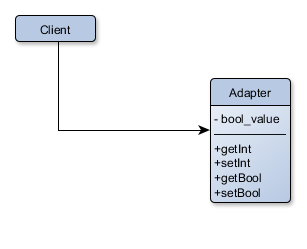
\includegraphics[width=0.64\textwidth]{./Adapter/Class/ClassDiagram.png}
	\caption{Class Adapter: Class Diagram }
	\label{CAclassDiag}
\end{figure}

\begin{itemize}
	\item \textbf{Adaptee}: legacy class with specific methods and fields
	\item \textbf{Target}: desired interface
	\item \textbf{ClassAdapter}: inherits from both Adaptee and Target, adapts the legacy methods to the desired interface  
\end{itemize}

\subsubsection{Fault Model}
Given that the pattern focuses on allowing access to legacy methods through a new interface, failures are found in the following situations:  
\begin{itemize}
	\item the adapter did not inherit from the legacy class or the new interface
	\item the adapter cannot interact with the legacy methods or unexpected results are produced
\end{itemize}

\subsection{Testing}
The two sources of failure both depend on the inability of the Client to reach the Adaptee methods through the Adapter.  We reasoned that it is thus sufficient to test the ways in which the variable \textit{bool\_value} interacts and is modified by the methods.
 As long as the variable changes in an unexpected way the connection between Client and Adaptee is in fact cut off.

We have represented the field's interaction with the class methods through a data flow graph in which the granularity was set to the level that basic blocks represent functions.

We then decided to test the interaction between the variable and the methods following the\textit{ all-uses} criterion, we in fact deemed the\textit{ all-def} criterion not useful to test this pattern because we value mainly the transmission of the right value of the field and thus find the need to test all its \textit{uses}.    


\paragraph{Data Flow Graph}
 The Client is the only external class interacting with the public methods of the Adapter. The Data Flow Graph can be seen in Figure \ref{CAdataflow}.
\begin{figure}[h]
	\centering
	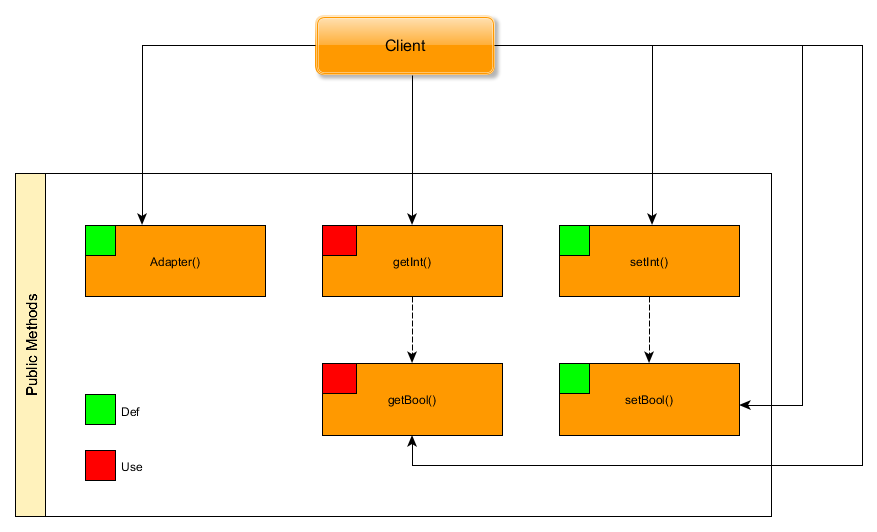
\includegraphics[width=0.84\textwidth]{./Adapter/Class/CallGraph.png}
	\caption{Data Flow Graph: \textit{bool\_value}}
	\label{CAdataflow}
\end{figure}


\subsubsection{Tests}
We generated a test suite capable of testing all the \textit{all-uses} paths:
\begin{itemize}
	\item Adapter() getInt() 
	\item Adapter() getBool() 
	\item Adapter() setInt() getInt() 
	\item Adapter() setInt() getBool() 
	\item Adapter() setBool() getInt()
	\newline
\end{itemize}
The special case of
\begin{itemize}
	\item Adapter() setBool() getBool() 
		
\end{itemize}	
is not tested because all the methods are directly inherited from the legacy class(and thus are supposedly already tested) and no side-effects, which could have invalidated some invariants, are introduced in our adapter.

In this particular pattern the absence of any external other than the Client class interacting in any way with the Adapter makes Unit and Integration tests un-distinguishable.

\subsubsection{Code Coverage}
The code coverage measure obtained from EclEmma Java plug-in is: 100\%.

%%%%%%%%%%%%%%%%%%%%%%%%%%%%%%%%%%%%%%%%%%%%%1
\newpage
\section{Object Adapter}
Adapts a pre-existent class to a new interface through class composition. 

Through the new interface the old methods can be directly presented, modified and produce aggregated results; completely new functionality can also be added. 
 

The composition adds the possibility of dynamically switching the adapted legacy class (not contemplated in our implementation) and the possibility of having overridden methods with altered functionality.

If the Adaptee class is declared final, the increased complexity from overridden methods is eliminated but the extra functionality is removed as well.


\subsubsection{Class Diagram}
\begin{figure}[!h]
	\centering
	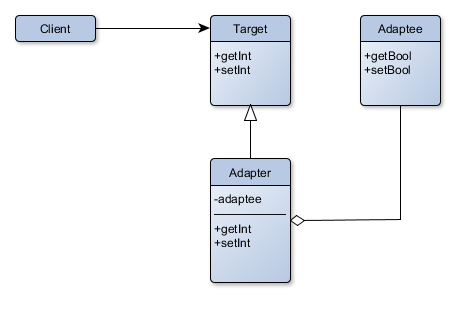
\includegraphics[width=0.7\textwidth]{./Adapter/Object/ClassDiagram.png}
	\caption{Object Adapter: Class Diagram }
	\label{OAclassDiag}
\end{figure}

\begin{itemize}
	\item \textbf{Adaptee}: legacy class with specific methods and fields
	\item \textbf{Target}: desired interface
	\item \textbf{ObjectAdapter}: inherits from Target, adapts the legacy methods to the desired interface through delegation
\end{itemize}

\subsubsection{Fault Model}
Given that the pattern focuses on allowing access to legacy methods through a new interface, failures are found in the following situations:  
\begin{itemize}
	\item the adapter did not inherit from the legacy class or the new interface
	\item the adapter cannot interact with the legacy methods 
	\item the instance contained in the adapter, which inherited the adaptee class, has overrode its methods in an unforeseen way
\end{itemize}


\subsection{Testing}

The sources of failure depend on the inability of the Client to reach the Adaptee methods through the Adapter or in the inability of the Adapter in foreseeing the possible ways in which the Adaptee methods can be overridden:  we reasoned that it is sufficient to test the ways in which the variable \textit{bool\_value} interacts and is modified by the methods, considering all the existent alternative implementations in the overridden methods. 
As long as the variable changes in an unexpected way the connection between Client and Adaptee is in fact cut off.

The problem of testing thus expands in two different orthogonal dimensions: data flow, the series of calls that modify or use the variable \textit{bool\_value},  and topology, the different ways the classes are ordered in a hierarchy at runtime.

We decided to explore both of them separately in specific focused tests.
\newline
\paragraph{Data Flow: field \textit{adaptee}}
We have represented the field's interaction with the class methods through a data flow graph in which the granularity was set such that basic blocks represent functions.

\subparagraph{Data Flow Graph}
Like the ClassAdapter, only the Client interacts with the Adapter methods.
The Data Flow Graph can be seen in Figure \ref{OAdataflow}.
\begin{figure}[!h]
	\centering
	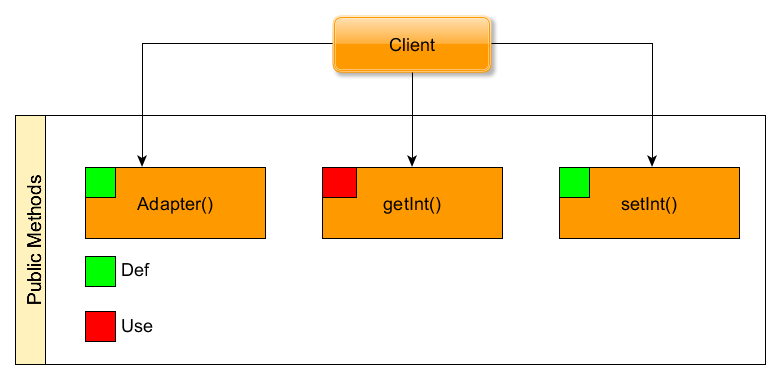
\includegraphics[width=0.84\textwidth]{./Adapter/Object/CallGraph.png}
	\caption{Data Flow Graph: \textit{bool\_value}}
	\label{OAdataflow}
\end{figure}


We then decided to test the interaction between the variable and the methods following the\textit{ all-uses} criterion, in this case it is identical to the \textit{all-def} criterion since there is only a single \textit{use}.   

\paragraph{Overridden methods}
We have tested separately in all the possible topologies exclusively the methods which presented overridden variants, without considering the methods which did not differ.

We reasoned that such a separation would allow us to sufficiently cover the code while maintaining a low number of tests.

\subsubsection{Tests}



We generated a test suite capable of testing all the \textit{all-uses} paths:
\begin{itemize}
	\item Adapter() getInt() 
	\item Adapter() setInt() getInt() 
	
\end{itemize}
To these are also added the topology tests:
\begin{itemize}
	\item Adapter( Adaptee ) getInt() 
	\item Adapter( AdapteeOpposite ) getInt()
\end{itemize}	
Of these the first, being already tested in the first suite, is not repeated.

Since in this pattern the tested class's methods (Adapter's) interacted with external classes (Adaptee) we  differentiated between Unit and Integration tests.

We utilized Mockito's \textit{mock} function to isolate errors with an origin in external classes from interfering with the Adapter class's code.
\subsubsection{Code Coverage}
The code coverage measure obtained from EclEmma Java plug-in is: 98.6\% 
\begin{itemize}
	\item Adapter: 97.1\% (UnitTest: 97.1\%)
	\item Adaptee: 100\%
	\item AdapteeOpposite: 100\% 
\end{itemize}

The single remaining untested branch is a setter method which was not called with all the possible inputs equivalence classes.

Since the Unit Tests and the Integration Tests are identical, with the only difference that the Unit Tests utilize Mockito's help to isolate from external classes, the coverage of the Adapter class's code is the same.

%%%%%%%%%%%%%%%%%%%%%%%%%%%%%%%%%%%%%%%%%%%%%2
 \newpage
\section{Proxy}

The Proxy pattern is constituted by a class  functioning as an interface to something else, usually a complex or heavy object.

 It is called by the client to access the real serving object behind the scenes, it either provides a cached result or transmits the request to the actual object.

\subsubsection{Class Diagram}
\begin{figure}[!h]
	\centering
	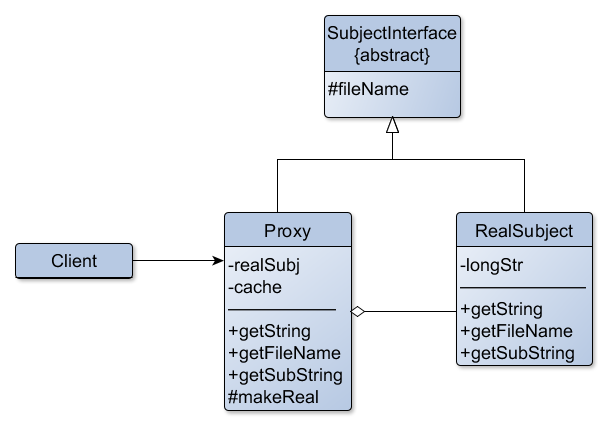
\includegraphics[width=0.79\textwidth]{./Proxy/ClassDiagram.png}
	\caption{Proxy: Class Diagram }
	\label{ProclassDiag}
\end{figure}

\begin{itemize}
	\item \textbf{SubjectInterface}: defines the interface used by the Client to access the RealSubject
	\item \textbf{Proxy}: allows access to the RealSubject, either by providing a cached response or by delegating the requests to the RealSubject itself
	\item \textbf{RealSubject}: defines the real complex or heavy object wrapped by the proxy
\end{itemize}

\subsubsection{Fault Model}

The pattern focuses on optimizing or controlling the access to the heavy subject. We have failures in the following situations:  
\begin{itemize}
	\item the access to the RealSubject is impeded
	\item the cached copies provided by the Proxy differ from the actual source.
\end{itemize}

\subsection{Testing}

The sources of failure depend on the inability of the Client to reach the RealSubject fields through the Proxy or on the inability of the Proxy of providing correct cached versions:  we reasoned that it is sufficient to test the ways in which the variable \textit{realSubj} interacts and is modified by the methods, by slight modification of the tests we can automatically verify the cached versions validity.




\paragraph{Data Flow: field \textit{realSubj}}
We have represented the field's interaction with the class methods through a data flow graph in which the granularity was set such that basic blocks represent functions.

\subparagraph{Data Flow Graph}
Only the Client interacts with the Proxy methods.
The Data Flow Graph can be seen in Figure \ref{Prodataflow}.
\begin{figure}[!h]
	\centering
	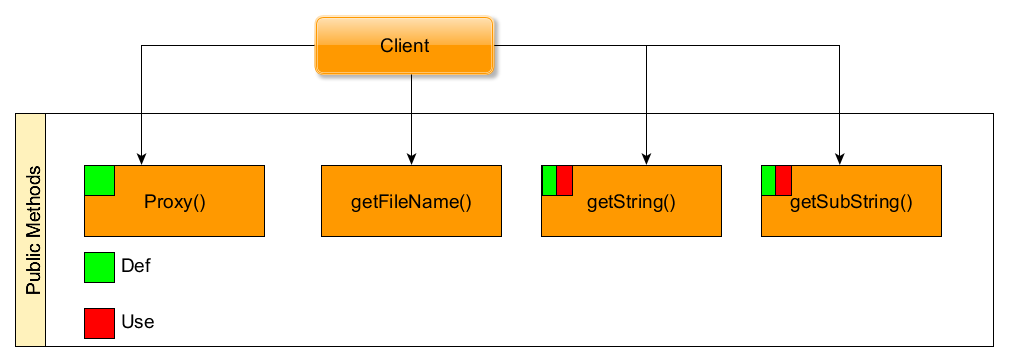
\includegraphics[width=0.94\textwidth]{./Proxy/CallGraph.png}
	\caption{Data Flow Graph: \textit{realSubj}}
	\label{Prodataflow}
\end{figure}


We decided to test the interaction between the variable and the methods following the\textit{ all-uses} criterion, we in fact desired to verify through the tests not only the correct interactions of the \textit{realSubj} field with the methods but also the \textit{cache}'s: we determined that a more extensive coverage could thus be desired.

\subsubsection{Tests}

\paragraph{Data Flow: field \textit{realSubj}}
We generated a test suite capable of testing all the \textit{all-uses} paths:
\begin{itemize}
	\item Proxy() getString() 
	\item Proxy() getString() getString()
	\item Proxy() getSubString()
	\item Proxy() getString() getSubString()
	\item Proxy() getSubString() getSubString()
	\item Proxy() getSubString() getString()
	
\end{itemize}
In particular  \textit{Proxy() getSubString() getSubString()} was altered to test the returned cached version after each method call. 


Since in this pattern the tested class's methods (Proxy's) interacted with external classes (RealSubject) we  differentiated between Unit and Integration tests.

There are difficulties in injecting mocked versions of the RealSubject in the Proxy.
The Proxy class, when called, has to provide a cached response or must instantiate a RealSubject which will process the data and report back: this means the instantiation happen directly inside the methods of the class, which means that, for testability, they must be altered to allow "outside interference" . 

Two possibilities were considered: create a RealSubject's Factory to pass during the construction of the Proxy and utilize it during the instantiation of the inner RealSubject or separate the responsibility of instantiation in a method void of logic.

In the first possibility, one would have to use Mockito's \textit{mock} method to mock the Factory so that it would return a mocked RealSubject, while in the second case one would have to use Mockito's \textit{spy} method to modify the Proxy itself so that the logic-less method would return a mocked RealSubject.

Due to not having to create an unnecessary extra class we preferred and thus implemented the second option.

\subsubsection{Code Coverage}
The code coverage measure obtained from EclEmma Java plug-in is: 93.8\% 
\begin{itemize}
	\item Proxy: 95.4\% (UnitTest 95.4\%)
	\item RealSubject: 88\%
	\item SubjectInterface: 100\%
	
\end{itemize}

The remaining untested branches correspond to the \textit{getFilename()} methods, which where not tested due to absence of logic.

Since the Unit Tests and the Integration Tests are identical, with the only difference that the Unit Tests utilize Mockito's help to isolate from external classes, the coverage of the Proxy class's code is the same.
%%%%%%%%%%%%%%%%%%%%%%%%%%%%%%%%%%%%%%%%%%%%%3
\section{Decorator}

The Decorator pattern allows behavior to be added to an individual object, either statically or dynamically, without affecting the behavior of other objects from the same class.
 

\subsubsection{Class Diagram}
\begin{figure}[!h]
	\centering
	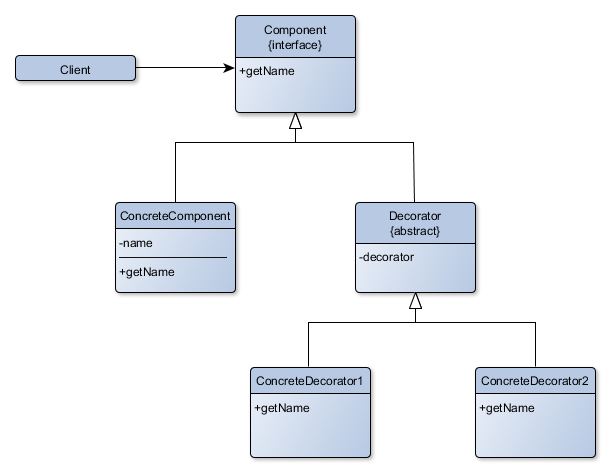
\includegraphics[width=0.79\textwidth]{./Decorator/ClassDiagram.png}
	\caption{Decorator: Class Diagram }
	\label{DeclassDiag}
\end{figure}

\begin{itemize}
	\item \textbf{Component}: common interface to the concrete component and its wrappers
	\item \textbf{ConcreteComponent}: implements the object to which responsibilities can be added
	\item \textbf{Decorator}: interface to concrete additive responsibilities, maintains a reference to a Component
	\item \textbf{ConcreteDecorator}: implements an additive responsibility
	
\end{itemize}
 
\subsubsection{Fault Model}

The pattern focuses on allowing an extension of functionality in objects. Grave errors are found in the following situations:  
\begin{itemize}
	\item the call to the \textit{operation (getName)} does not reach the Component or results in unexpected behavior
\end{itemize}


\subsection{Testing}

The sources of failure depend on the presence of errors in the sequence of additive behavior to the \textit{operation (getName)}. We reasoned that to produce a satisfying test suite it is sufficient to test the correctness of the sequence of method calls in different hierarchies of classes.

\paragraph{Topology: method \textit{operation()}}
We generated a Class Dependency Graph to identify all the possible relations between classes.

\subparagraph{Class Dependency Graph}
In the Figure \ref{Dedepengraph} are made explicit the relations between classes: in particular, since Decorator is an abstract class, it and its inheriting classes depend on each other. 
\begin{figure}[!h]
	\centering
	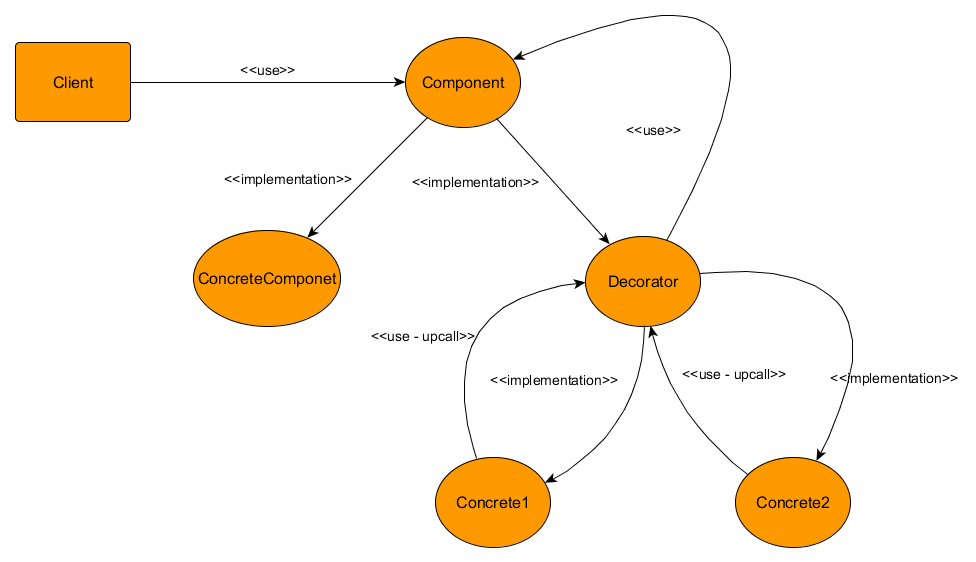
\includegraphics[width=1\textwidth]{./Decorator/ClassDepencyGraph.png}
	\caption{Class Dependency Graph: \textit{getName()}}
	\label{Dedepengraph}
\end{figure}

We decided to generate a test suite dependent on the \textit{all-edges} criterion.

\subsubsection{Tests}
\paragraph{Topology: method \textit{operation()}}
We identified the 3 cases of:
\begin{itemize}
	\item ConcreteComponent
	\item Decorator ConcreteComponent
	\item Decorator Decorator ConcreteComponent
	
\end{itemize}
as representative of the entire set of possible hierarchies.
We then tested the \textit{getName()} method on the identified cases.
Technically for the \textit{all-edges} criterion the third test would have been enough, but we decided to be more rigorous and test for all the possible equivalence classes of topologies.


Since the tested class's methods (ConcreteComponent and Decorator) interacted with external classes (an other Component) we  differentiated between Unit and Integration tests.

We utilized Mockito's \textit{mock} function to isolate errors with an origin in external classes from interfering with the main class's code.
\subsubsection{Code Coverage}
The code coverage measure obtained from EclEmma Java plug-in is: 100\% (Unit: 100\%) 


Since the Unit Tests and the Integration Tests are identical, with the only difference that the Unit Tests utilize Mockito's help to isolate from external classes, the coverage of the classes' code is the same.

%%%%%%%%%%%%%%%%%%%%%%%%%%%%%%%%%%%%%%%%%%%%%4
\section{Composite}

The Composite pattern "composes" objects into tree structures to represent part-whole hierarchies. Implementing the composite pattern lets clients treat individual objects and compositions uniformly.

\subsubsection{Class Diagram}
\begin{figure}[!h]
	\centering
	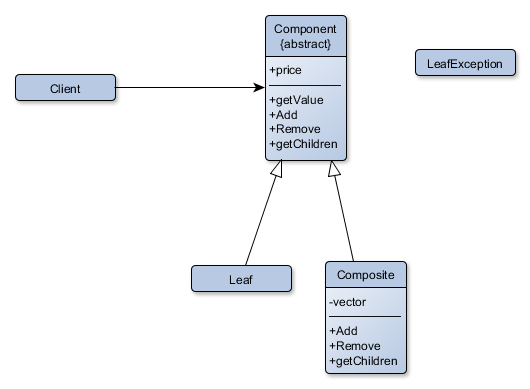
\includegraphics[width=0.89\textwidth]{./Composite/ClassDiagram.png}
	\caption{Composite: Class Diagram }
	\label{CoclassDiag}
\end{figure}

\begin{itemize}
	\item \textbf{Component}: common interface to the individual and compound objects
	\item \textbf{Composite}: composition of individual objects and other compositions
	\item \textbf{Leaf}: individual object
	\item \textbf{LeafException}: exception thrown when a composite-specific method is called on a Leaf object
		
\end{itemize}

\subsubsection{Fault Model}

The pattern focuses on treating uniformly individual and compound objects. Grave errors are found in the following situations:  
\begin{itemize}
	\item the common \textit{operation} works differently than expected
	\item the composite-specific methods produce unexpected results when called on a Leaf object
\end{itemize}


\subsection{Testing}

The sources of failure depend on the inability of the specific components (individual or composite parts) to be interacted in an uniform way. We reasoned that to produce a satisfying test suite we must test two different things: the way \textit{operation} works under the possible hierarchies at runtime and the way the different objects behave under calls from composite-specific methods.

As long as outcomes different from the expectation are observed we can reasonably predict that no uniform treatments of the components is in place.

The problem of testing thus expands in two different orthogonal dimensions: data flow, the series of calls that modify or use the variable \textit{price},  and topology, the different hierarchies of objects with respect to the method \textit{operation}.


We decided to explore both of them separately in specific focused tests.

\paragraph{Data Flow: field \textit{price}}
We have represented the field's interaction with the class methods through a data flow graph in which the granularity was set such that basic blocks represent functions.

\subparagraph{Data Flow Graph}
Both Client and other wrapping Composites interacts with the Component methods.
The Data Flow Graph can be seen in Figure \ref{Codataflow}.
\begin{figure}[!h]
	\centering
	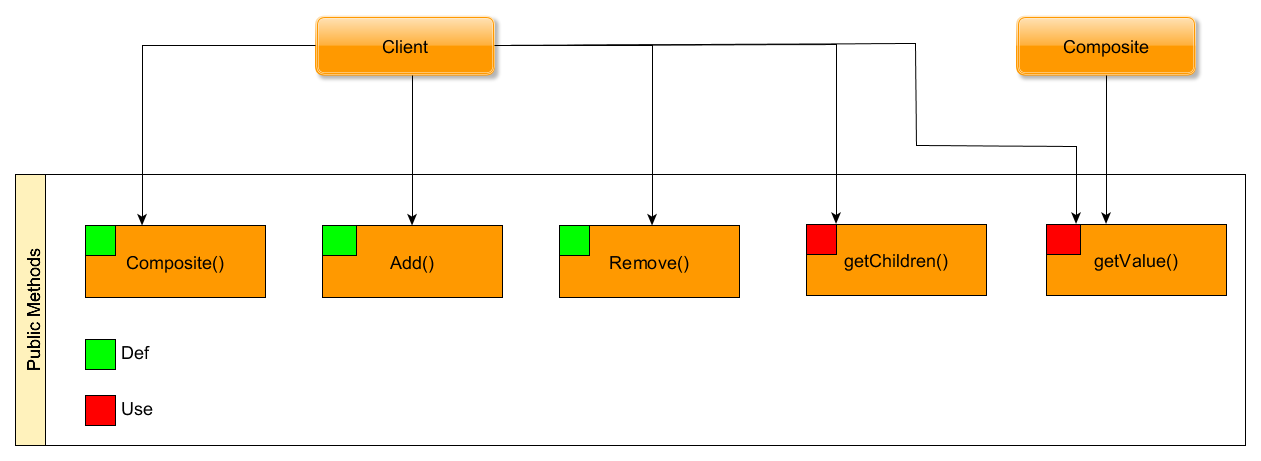
\includegraphics[width=1\textwidth]{./Composite/CallGraph.png}
	\caption{Data Flow Graph: \textit{price}}
	\label{Codataflow}
\end{figure}


We decided to test the interaction between the variable and the methods following the\textit{ all-uses} criterion, we deemed the \textit{all-def} criterion excessively restrictive to test this pattern.

The field was tested in the fixed hierarchy formed with a Composite element containing another Composite, which contained a Leaf.  
We reasoned that the chosen fixed hierarchy, while not allowing to test on each possible instance, is sufficiently complete, maintaining a balance between number of tests and efficiency.
  
  
  
\paragraph{Topology: methods \textit{composition-specific}}
We generated a Class Dependency Graph to identify all the possible relations between classes.

\subparagraph{Class Dependency Graph}
In the Figure \ref{Codepengraph} are made explicit the relations between classes: in particular since Component is an abstract class it and its inheriting classes depend on each other. 
\begin{figure}[!h]
	\centering
	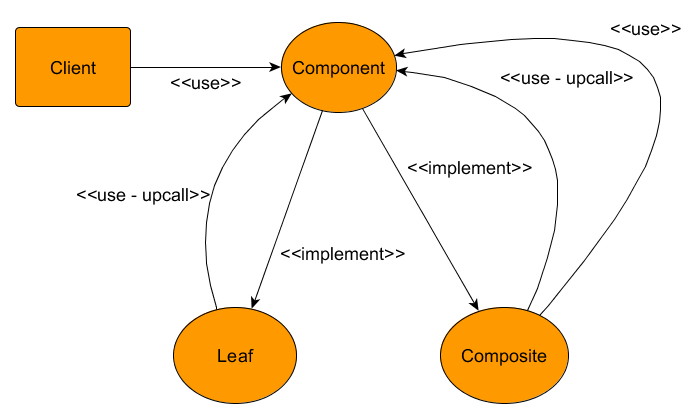
\includegraphics[width=0.8\textwidth]{./Composite/ClassDepencyGraph.png}
	\caption{Class Dependency Graph: \textit{composition-specific}}
	\label{Codepengraph}
\end{figure}

We decided to generate a test suite dependent on the \textit{all-edges} criterion.\textit{ all-nodes} is in fact excessively relaxed and would not cover all cases of interests. 

\subsubsection{Tests}

\paragraph{Data Flow: field \textit{price}}
We generated a test suite capable of testing all the \textit{all-uses} paths:
\begin{itemize}
	\item Component() getChild()
	\item Component() getValue()
	\item Component() add() getChild()
	\item Component() add() getValue()
	\item Component() add() add() remove() getChild()
	\item Component() add() add() remove() getValue() 
\end{itemize}

\paragraph{Topology: methods \textit{composition-specific}}
We identified the 3 cases of:
\begin{itemize}
	\item single Leaf
	\item Composite containing Leaf
	\item Composite containing Composite
\end{itemize}
as representative of the entire set of possible hierarchies.

We then tested all the composite-specific methods (add, remove, getChild) on the identified cases.

In both type of tests, since the tested class's methods (Component) interacted with external classes (Leaf or Composites) we  differentiated between Unit and Integration tests.

We utilized Mockito's \textit{mock} function to isolate errors with an origin in external classes from interfering with the main class's code.
\subsubsection{Code Coverage}
The code coverage measure obtained from EclEmma Java plug-in is: 97.8\% 
\begin{itemize}
	\item Component: 92.3\% (UnitTest 92.3\%)
	\item Composite: 100\%
	\item Leaf: 100\%
	\item LeafException 100\%
\end{itemize}

The remaining untested branches are found in the implementation of the composite-specific methods that Component provides for Leaf: all other classes (Composite) directly override those methods so their implementation, when they are called not by a Leaf, is never tested.

Since the Unit Tests and the Integration Tests are identical, with the only difference that the Unit Tests utilize Mockito's help to isolate from external classes, the coverage of the classes' code is the same.


%%%%%%%%%%%%%%%%%%%%%%%%%%%%%%%%%%%%%%%%%%%%%5
\section{Observer}

In the Observer pattern an object, called the subject, maintains a list of its dependents, called observers, and notifies them automatically of any state changes, usually by calling one of their methods.

The observers must be explicitly associated and disassociated with the subjects they follow, possibly causing memory leaks.

\subsubsection{Class Diagram}
\begin{figure}[!h]
	\centering
	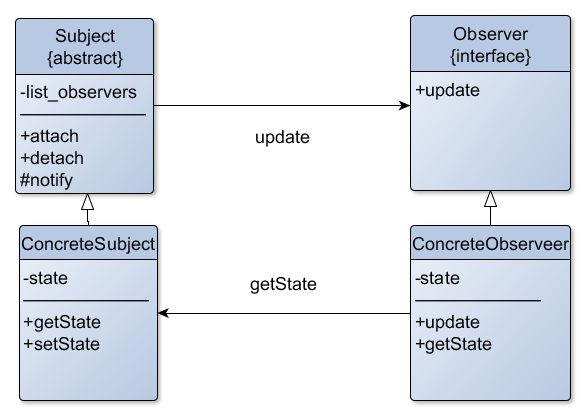
\includegraphics[width=0.8\textwidth]{./Observer/ClassDiagram.png}
	\caption{Observer: Class Diagram }
	\label{ObclassDiag}
\end{figure}

\begin{itemize}
	\item \textbf{Subject}: provides methods to add or remove observers in his list of followers
	\item \textbf{Observer}: specifies an interface for the notification of change on a subject
	\item \textbf{ConcreteSubject}: contains a state that can be modified
	\item \textbf{ConcreteObserver}: implements the update operation
	
\end{itemize}

\subsubsection{Fault Model}

The pattern focuses on maintaining updated objects that expressed the interest in a specific subject. Failures are found in the following situations:  
\begin{itemize}
	\item \textit{attach} and \textit{detach} do not produce the expected results.
	\item after a change of the subject state the dependent observers are not \textit{notified}.
	\item the observer after being notified does not execute correctly the \textit{update} method.
\end{itemize}


\subsection{Testing}

The sources of failure depend on the presence of problems that impede the correct functioning of the inter-class methods and, in the lesser part, by the inability of the observer to correctly update. We considered the correct modification on the subject internal \textit{state} as not important for our pattern.  We reasoned that to produce a satisfying test suite we must test the way \textit{list\_observers} is modified after an inter-class method invocation and the way the \textit{state} of the observer is modified after a notification.



As long as the outcomes differ from the expectation we can reasonably predict that the transmission of information upon notification encountered problems.

\paragraph{Data Flow: field \textit{list\_observers}}
We have represented the field's interaction with the class methods through a data flow graph in which the granularity was set such that basic blocks represent functions.

\subparagraph{Data Flow Graph}
Only the Client interacts with the Subject methods, in particular the responsibility of attaching or detaching Observers from Subjects lies with the Client.
The Data Flow Graph can be seen in Figure \ref{Obdataflow1}.
\begin{figure}[!h]
	\centering
	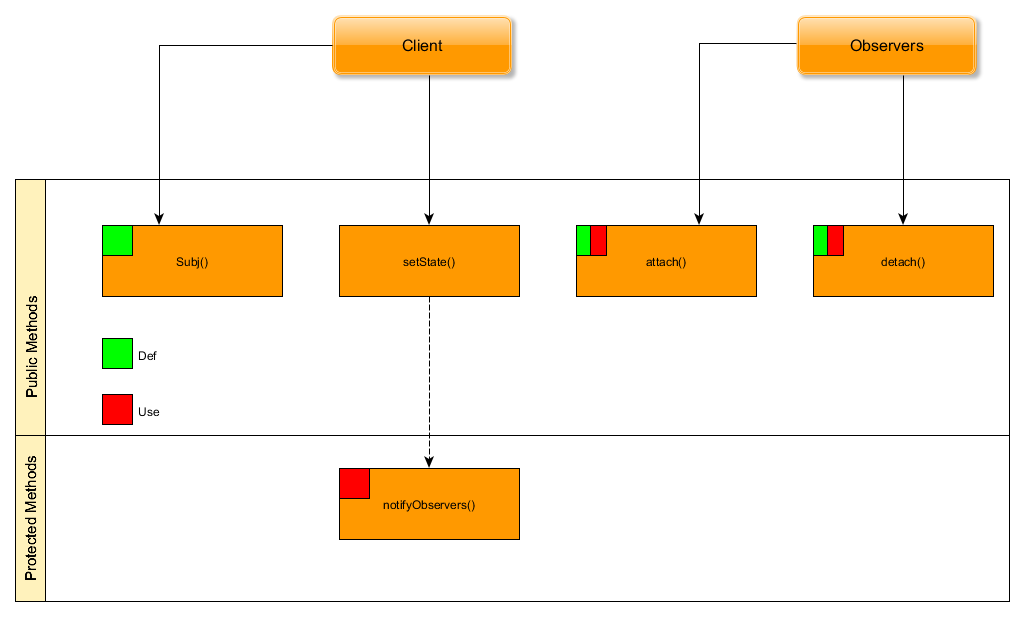
\includegraphics[width=1\textwidth]{./Observer/CallGraph.png}
	\caption{Data Flow Graph: \textit{list\_observers}}
	\label{Obdataflow1}
\end{figure}


We decided to test the interaction between the variable and the methods following the\textit{ all-uses} criterion.

\paragraph{Data Flow: field \textit{state}}
We have represented the field's interaction with the class methods through a data flow graph in which the granularity was set such that basic blocks represent functions.

\subparagraph{Data Flow Graph}
Both Client and followed Subjects interacts with the Component methods.
The Data Flow Graph can be seen in Figure \ref{Obdataflow2}.
\begin{figure}[!h]
	\centering
	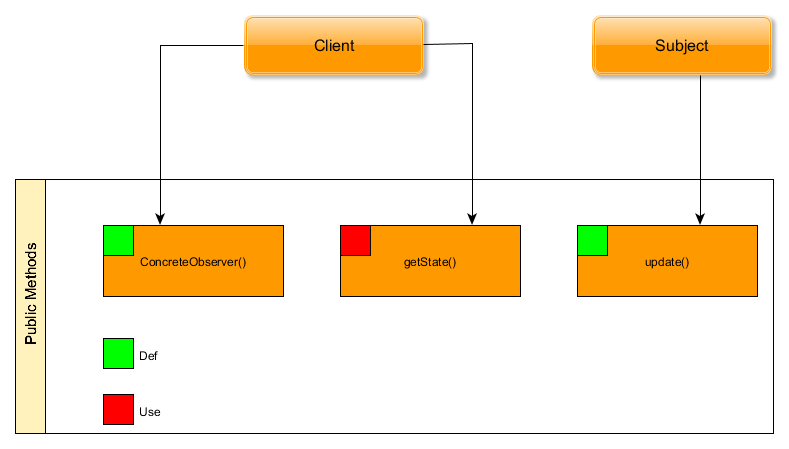
\includegraphics[width=0.9\textwidth]{./Observer/CallGraph_State.png}
	\caption{Data Flow Graph: \textit{state}}
	\label{Obdataflow2}
\end{figure}


We decided to test the interaction between the variable and the methods following the\textit{ all-uses} criterion, we deemed the \textit{all-def} criterion excessively restrictive to test this pattern.


\subsubsection{Tests}

\paragraph{Data Flow: field \textit{list\_observer}}
We decided to test as separate and distinct cases for situations like \textit{detach() detach()} where the methods are called with the same Observer or different ones. 
We generated a test suite capable of testing all the \textit{all-uses} paths:
\begin{itemize}
	\item Subject() setState()[notify()]	
	\item Subject() detach() 		
	\item Subject() attach()x3 detach()x2 (+setState()[notify()]) 
	\item Subject() attach()x2 detach()x2 attach() detach() attach() (+setState()[notify()])
\end{itemize}
\vspace{3mm}

Each of these paths is interesting for more in-depth study:
\begin{enumerate}
	\item controls no errors are introduced if a \textit{setState()} is called with empty list
	\item a detach is called with empty list
	\item[3,4] by interspersing verifications on the \textit{list\_observer} we test all combinations of the different D-U paths:
	\begin{enumerate}
		\item[-] attach() attach()  
		\item[-] attach() detach()	 	
		\item[-] detach() detach()	 
		\item[-] detach() notify()
		\item[-] Subject() attach()
		\item[-] detach() attach()
		\item[-] attach() notify()
	\end{enumerate} 
	
\end{enumerate} 
To create an output of the \textit{list\_observer} we utilize a support method void of logic, which we decided did not need to be considered as an \textit{use} during the tests.


\paragraph{Data Flow: field \textit{state}}
We generated a test suite capable of testing all the \textit{all-uses} paths:
\begin{itemize}
	\item ConcreteObserver() getState()
	\item ConcreteObserver() update() getState()
	
\end{itemize}
	

\vspace{6mm}	

In testing both fields, since the tested class's methods (ConcreteSubject and ConcreteObserver) interacted with external classes (Observer and Subject) we  differentiated between Unit and Integration tests.

We utilized Mockito's \textit{mock} function to isolate errors with an origin in external classes from interfering with the main class's code.

\subsubsection{Code Coverage}
The code coverage measure obtained from EclEmma Java plug-in is: 100\% (Unit: 100\%)

\newpage
%%%%%%%%%%%%%%%%%%%%%%%%%%%%%%%%%%%%%%%%%%%%%6
\section{State}

The State pattern implements a state machine by implementing each individual state as a derived class of the state pattern interface, and implementing state transitions by invoking methods defined by the pattern's superclass.

\subsubsection{Class Diagram}
\begin{figure}[!h]
	\centering
	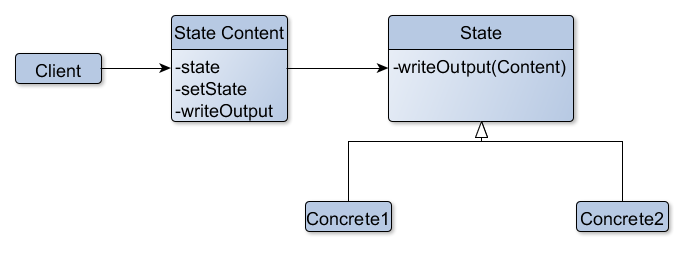
\includegraphics[width=0.9\textwidth]{./State/ClassDiagram.png}
	\caption{State: Class Diagram }
	\label{SclassDiag}
\end{figure}

\begin{itemize}
	\item \textbf{StateContext}: maintains an instance of State to serve as its inner state
	\item \textbf{State}: interface of classes with the specific behavior desired by StateContext
	\item \textbf{ConcreteState}: implements StateContext's functions, possibly dependent on an inner state 
	
\end{itemize}

\subsubsection{Fault Model}
 
The pattern focuses on delegating the actual methods implementation to internal state classes. Grave errors are found in the following situations:  
\begin{itemize}
	\item internal state changes in an erroneous manner. 
	\item the internal state methods produce unexpected side effects or results.
	\item (with less importance) the internal classes' inner state changes in an erroneous manner.
\end{itemize}


\subsection{Testing}

The sources of failure are errors found in the internal classes methods. We reasoned that to produce a satisfying test suite it is sufficient to test the way the \textit{state} field interacts with the StateContext methods: by testing the field in fact we are also testing the way the instance's own methods are implemented.

We also decided to not rigorously test the way the ConcreteStates inner state is updated since we reasoned it is only a lesser error source.

\paragraph{Data Flow: field \textit{state}}
We have represented the field's interaction with the class methods through a data flow graph in which the granularity was set such that basic blocks represent functions.

\subparagraph{Data Flow Graph}
Both the Client and ConcreteStates methods interacts with the StateContext functions.
The Data Flow Graph can be seen in Figure \ref{Sdataflow}.
\begin{figure}[!h]
	\centering
	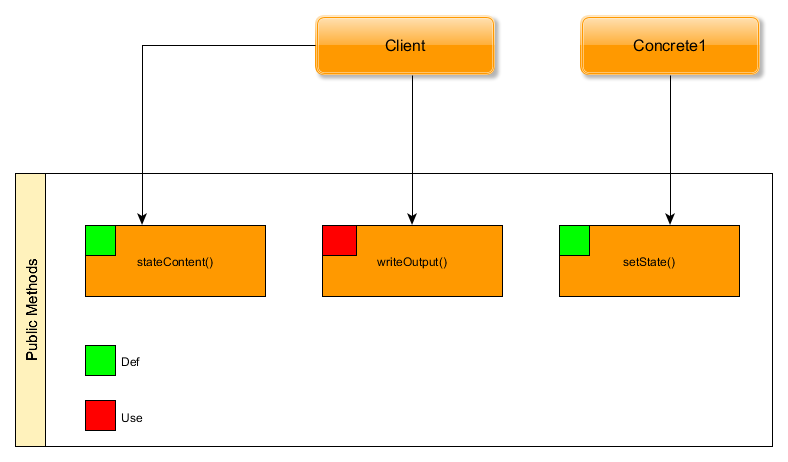
\includegraphics[width=0.8\textwidth]{./State/CallGraph.png}
	\caption{Data Flow Graph: \textit{state}}
	\label{Sdataflow}
\end{figure}


We decided to test the interaction between the variable and the methods following the\textit{ all-uses} criterion.

\subsubsection{Tests}

\paragraph{Data Flow: field \textit{state}}
We generated a test suite capable of testing all the \textit{all-uses} paths:
\begin{itemize}
	\item StateContext() writeOutput() 
	\item StateContext() setState() writeOutput()
	\item StateContext() writeOutput() writeOutput()
\end{itemize}

The last test case is actually used to test the correctness of the way ConcreteStates update the field and does not cover a particular D-U path. 
 

Since the tested class's methods (StateContext) interacted with external classes (ConcreteStates) we  differentiated between Unit and Integration tests.

We utilized Mockito's \textit{mock} function to isolate errors with an origin in external classes from interfering with the main class's code.
\subsubsection{Code Coverage}
The code coverage measure obtained from EclEmma Java plug-in is: 100\% (Unit: StateContext: 100\%) 


\newpage
%%%%%%%%%%%%%%%%%%%%%%%%%%%%%%%%%%%%%%%%%%%%%7
\section{Visitor}
The Visitor pattern is a way of separating an algorithm from an object structure on which it operates. 

The pattern allows one to add new virtual functions to a family of classes without modifying the classes themselves: the visitor class implements all of the appropriate specializations of the virtual function. The visitor takes the instance reference as input and produces the output through double dispatch.


\subsubsection{Class Diagram}
\begin{figure}[!h]
	\centering
	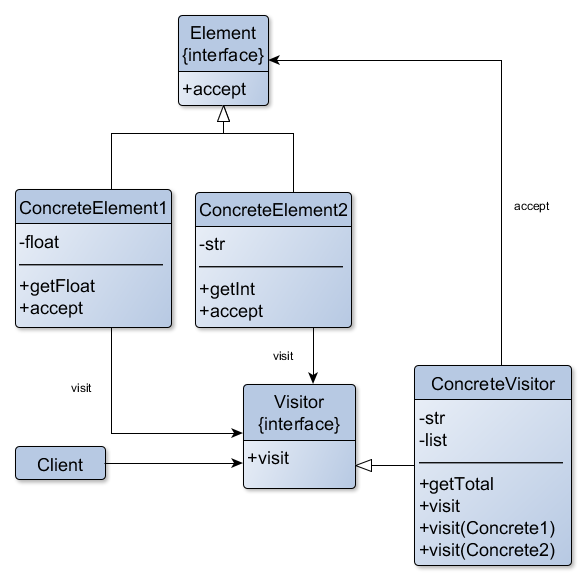
\includegraphics[width=1\textwidth]{./Visitor/ClassDiagram.png}
	\caption{Visitor: Class Diagram }
	\label{ViclassDiag}
\end{figure}

\begin{itemize}
	\item \textbf{Visitor}: interface to the concrete implementations
	\item \textbf{ConcreteVisitor}: implements the various specific way of visiting concrete elements, the actual way an element is visited is determined by the signature of the method called in the double dispatch
	\item \textbf{Element}: interface of visitable element
	\item \textbf{ConcreteElement}: contains specific fields and logic, is visitable
	
\end{itemize}

\subsubsection{Fault Model}

The pattern focuses on treating uniformly objects of different types while operating on them with different specializations of the same function. A failure is produced by the following situation:  
\begin{itemize}
	\item the wrong \textit{visit()} is applied to an Element
\end{itemize}


\subsection{Testing}

The sources of failure depend on the inability of the Visitor to identify the specialized implementation to execute. This depends mainly on the type of Element we are working with. We thus reasoned that to produce a satisfying test suite we must test the way \textit{visit} works when applied to all possible hierarchies of Element types.

\paragraph{Topology: method \textit{visit()}}
We generated a Class Dependency Graph to identify all the possible relations between classes.

\subparagraph{Class Dependency Graph}
In the Figure \ref{Videpengraph} are made explicit the relations between classes. 
\begin{figure}[!h]
	\centering
	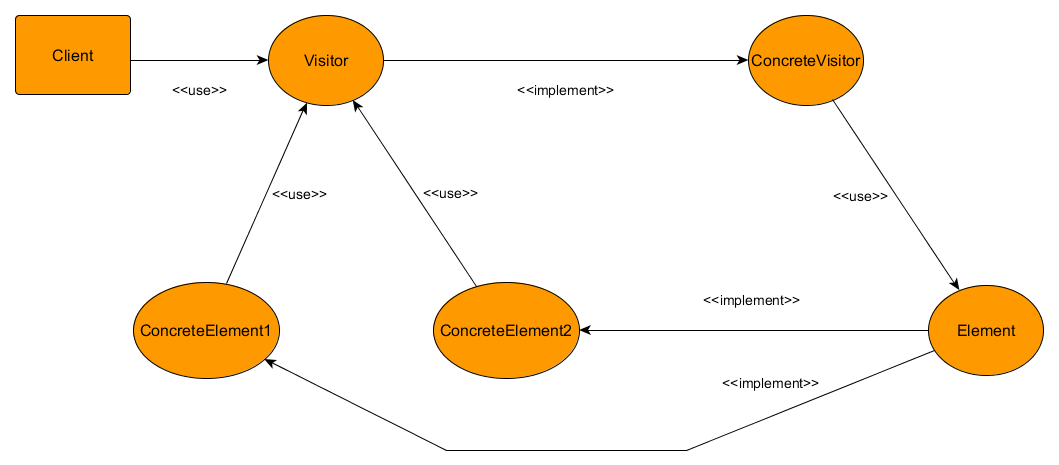
\includegraphics[width=1\textwidth]{./Visitor/ClassDependencyGraph.png}
	\caption{Class Dependency Graph: \textit{visit()}}
	\label{Videpengraph}
\end{figure}

We decided to generate a test suite dependent on the \textit{all-edges} criterion, in this case it is identical to the\textit{ all-nodes} criterion.

\subsubsection{Tests}
  	
\paragraph{Topology: method \textit{visit()}}
We identified the 2 cases:
\begin{itemize}
		\item Visitor ConcreteVisitor Element ConcreteElement2 Visitor
		\item Visitor ConcreteVisitor Element ConcreteElement1 Visitor	
\end{itemize}
as representative of the entire set of possible hierarchies.

Since in this pattern the tested class's methods (Visitor's) interacted with external classes (ConcreteElements) we  differentiated between Unit and Integration tests.

We utilized Mockito's \textit{mock} function to isolate errors with an origin in external classes from interfering with the main class's code.

In particular, we explored Mockito's functionalities and decided to utilize its Answer class to directly produce side-effects once the \textit{accept()} method was called, rather than mechanically calling the generalized \textit{visit()} and then the specialized version (or directly this second one). 
\subsubsection{Code Coverage}
The code coverage measure obtained from EclEmma Java plug-in is: 100\% (Unit: Visitor: 100\%)

Since the Unit Tests and the Integration Tests are identical, with the only difference that the Unit Tests utilize Mockito's help to isolate from external classes, the coverage of the classes' code is the same.

%%%%%%%%%%%%%%%%%%%%%%%%%%%%%%%%%%%%%%%%%%%%%8

\chapter{JUnit \& Mockito}
To generate and execute the test cases of our chosen test suites we utilized the already existent Java frameworks provided by JUnit\cite{1} and Mockito\cite{2}. To further provide a measure of code coverage we utilized the specific JUnit's plug-in EclEmma\cite{3}.

\section{JUnit}

JUnit is an open source unit testing framework for the Java programming language. JUnit has been important in the development of test-driven development and is one of a family of unit testing frameworks which is collectively known as xUnit that originated with SUnit.

JUnit is linked as a JAR at compile-time: the framework resides under package junit.framework for JUnit 3.8 and earlier, and under package org.junit for JUnit 4 and later: this allows JUnit 4 to maintain backward compatibility.
JUnit 5 is currently in its beta phase.

The framework allows the programmer to easily create \textit{drivers} for the tests and the ability to immediately verify the produced outputs. 

The tests, in fact, return a success if all the \textit{Assertion}s contained therein are verified.

In our project we utilized JUnit 4 for the added functionality it provides: \textit{Annotation}s to identify the test methods and a wider range of Assertions for testing expected results, among which an equality between Arrays which we utilized in our tests.

Main benefits of the framework are: \begin{itemize}
	\item JUnit tests can be run automatically, check their own results and provide immediate feedback without a need to manually comb through a report of test results.
	
	\item JUnit tests can be organized into test suites containing test cases and even other test suites.

	\item Junit shows test progress through an user-friendly bar that is green while the tests have not encountered errors and turns red when a test fails.

\end{itemize}

\section{Mockito}

Mockito is an open source testing framework for Java. The framework allows the creation of test double objects (mock objects) in automated unit tests for the purpose of Test-driven Development (TDD) or Behavior Driven Development (BDD).

Mock testing frameworks are utilized to lower the cost of testing: ensuring that objects perform the behaviors that are expected of them in fact requires the creation of test automation frameworks that actually exercises each behavior and verifies that it performs as expected. The problem is that the requirement to create an entire testing framework is often an onerous task that requires as much effort as writing the original objects that were supposed to be tested. 

Mock testing frameworks thus come to aid in effectively faking some external dependencies so that the object being tested has a consistent interaction with its outside dependencies, thus notably lowering the onus on the programmer.

While utilizing the framework we identified some noteworthy details:
\begin{itemize}
	\item in the Proxy class we utilized \textit{spy} on the very class we were testing to allow injection of other mocked classes
	\item  when using \textit{spy}, the \textit{doReturn().when()} construct is to be preferred to the \textit{when().myMethod()} construct due to the fact that the latter actually executes the function and produces side-effects before returning the designed output
	\item returning an Answer() allows for side-effects to be produced when a mocked object's method is called. 
	\item Answer is not necessary if the side-effects are produced only on the very class under test due to the fact that one can independently produce them by simply calling the respective tested methods.
\end{itemize}


 

\paragraph{EclEmma}
EclEmma is an open source toolkit for measuring and reporting Java code coverage for Eclipse. 
It does not require any kind of modification to the code and can work over tests executed in JUnit. 
EclEmma measures the branch coverage of the bytecode produced by the compiler. The branches which were not tested are then traced back to the code and highlighted as a warning. 

In some cases such highlighting is confusing and can even be impossible to eliminate through testing: the Java compiler in fact sometimes creates additional bytecode that seems to have no relation to the source code (e.g. synthetic classes and methods). 

In some other cases test execution is questionable or impossible by design: private, empty default constructors (assuming they receive no calls) or methods that contains no logic, like plain getters and setters,
or even extra exception handlers installed to close resources from try/with statements.

\addcontentsline{toc}{chapter}{\protect\numberline{}Conclusions}
\chapter*{Conclusions}
We identified a collection of structural and behavioral design patterns; for each pattern, we produced an implementation in Java, which we then studied to identify the main faults they were susceptible to.
We created a reasoned test suite based on the fault model and on a coverage criteria chosen pattern by pattern.

We realized both Unit and Integration tests through the JUnit\cite{1} plug-in for Eclipse and the Mockito\cite{2} framework; we then applied EclEmma\cite{3} to provide a code coverage measure.

This measure was subsequently studied to identify both the untested branches and the reason for which they were not covered.

In the end most patterns (except ObjectAdapter, Proxy and Composite) presented a full code coverage.

Even the lowest covered pattern, Proxy, presents a 93.8\% measure of code coverage, with the untested branches being lines of code void of logic. We can thus consider the possibility of relaxing the coverage criteria used: in testing modification of fields through data flow graphs, rather than applying an \textit{all-uses} criterion we could use an \textit{all-def}; in testing the correct delegation in different topologies (Class Dependency Graphs) we could substitute the \textit{all-nodes} criterion to the \textit{all-edges} we used.
 

\addcontentsline{toc}{chapter}{\protect\numberline{}The Bibliography}
\begin{thebibliography}{9}

\bibitem{4} E. Gamma, R. Helm, R. Johnson and J. Lasvergeres, \textit{Design Patterns}. Paris: Vuibert, 1999.
\bibitem{1} JUnit, \url{http://junit.org/junit4/javadoc/latest}, 1 Aug. 2016
\bibitem{2} Mockito, \url{http://site.mockito.org/mockito/docs/current/org/mockito/Mockito.html}, 1 Aug. 2016
\bibitem{3} EclEmma, \url{http://www.eclemma.org/index.html}, 1 Aug. 2016

\end{thebibliography}
\addcontentsline{toc}{chapter}{\protect\numberline{}List of Figures}
\listoffigures
\end{document}
